% !TeX encoding = UTF-8
% !TeX spellcheck = es_ES
% !TeX root = ../ComponentCatalog.tex
%!TEX root=../ComponentCatalog.tex

%DC Jack 2 mm plastico Amazon
\begin{table}[H]
    \centering
    \renewcommand\theadfont{\bfseries}
    \setlength{\tabcolsep}{10pt}
    \renewcommand{\arraystretch}{1.5}

    \begin{tabular}{|c|c|c|c|c|}
        \beginConnectorTable{DC Jack 2mm}
        \multirow{3}{*}{\makecell{Macho \\ Plug}}
    
        \connectordata{
            \begin{scope}
                \clip (-1.3,-0.75) rectangle  +(2.6,1.5);
                \node[inner sep=0pt] at (-1.8,-0.8)
                    {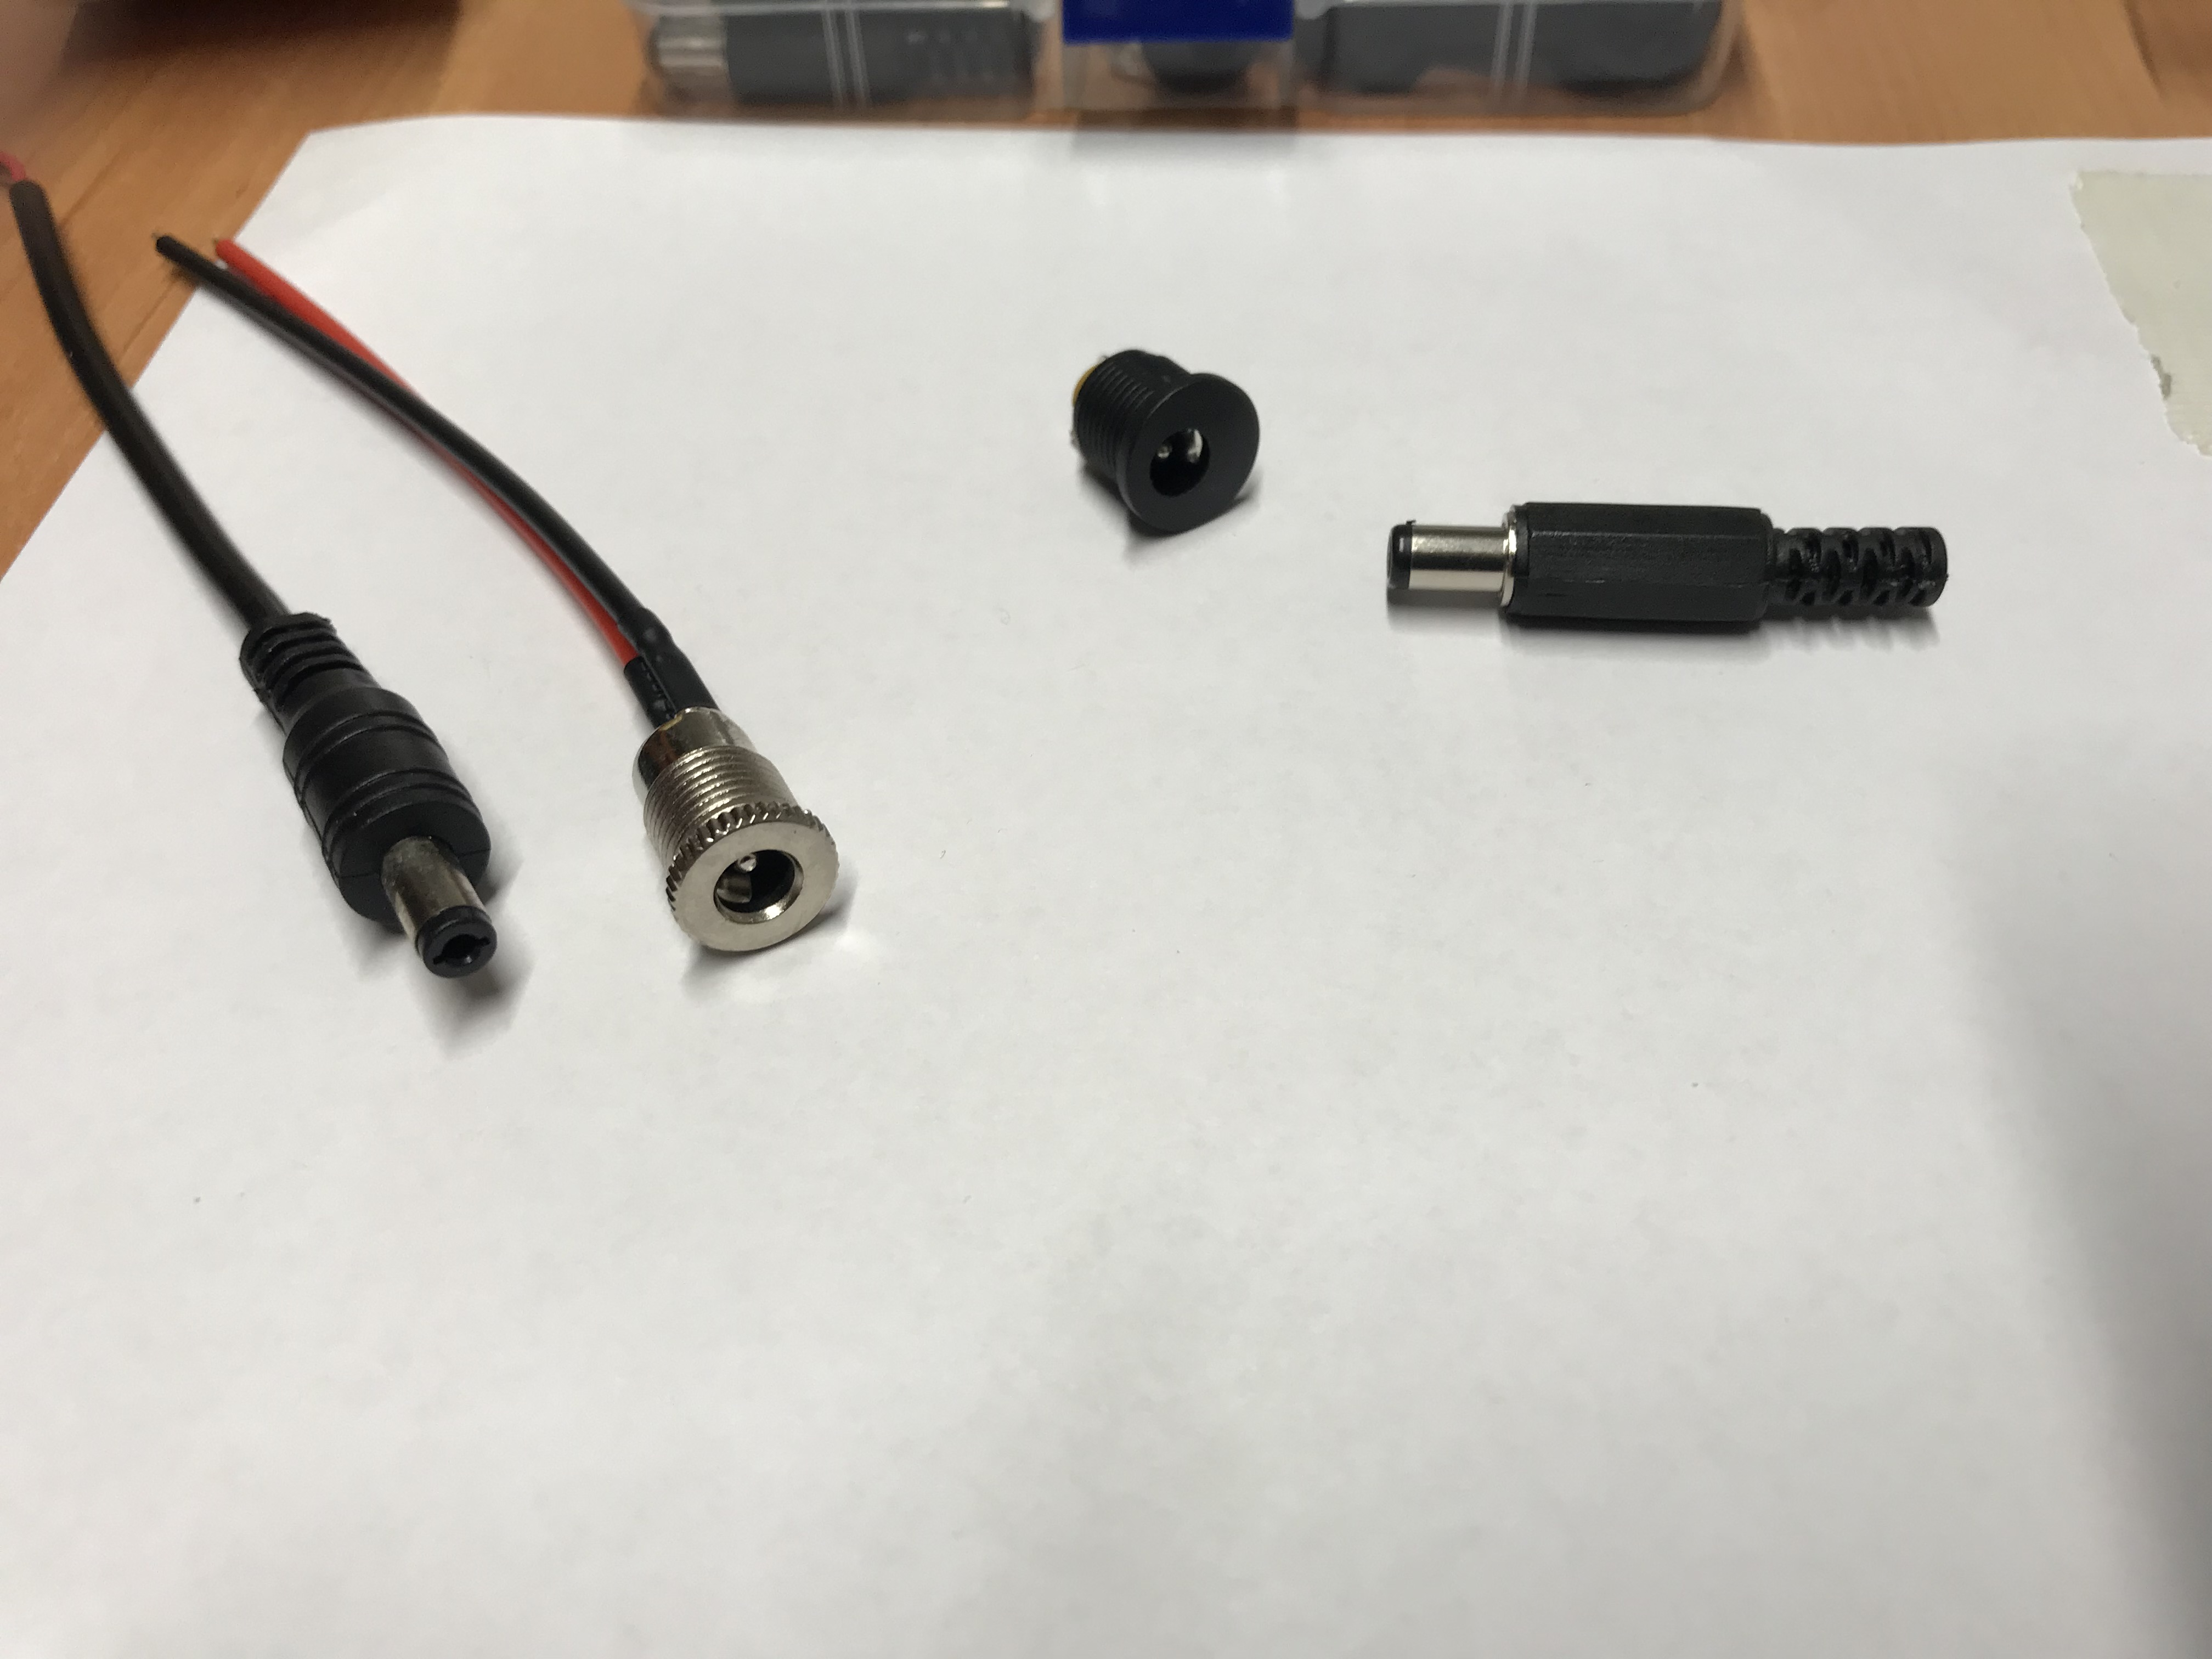
\includegraphics[scale=.05]{pictures/dcJack.jpg}};
            \end{scope}
        }{
            \draw (0,0) rectangle (3,1.5) ;
        }{Amazon}{Sin Id} {24V} {3A}
        \cline{1 - 2}
        \multirow{3}{*}{\makecell{Hembra \\ Socket}}
        \connectordata{
            \begin{scope}
                \clip (-1,-0.75) rectangle  +(2,1.5);
                \node[inner sep=0pt] at (-0.2,-1.7)
                    {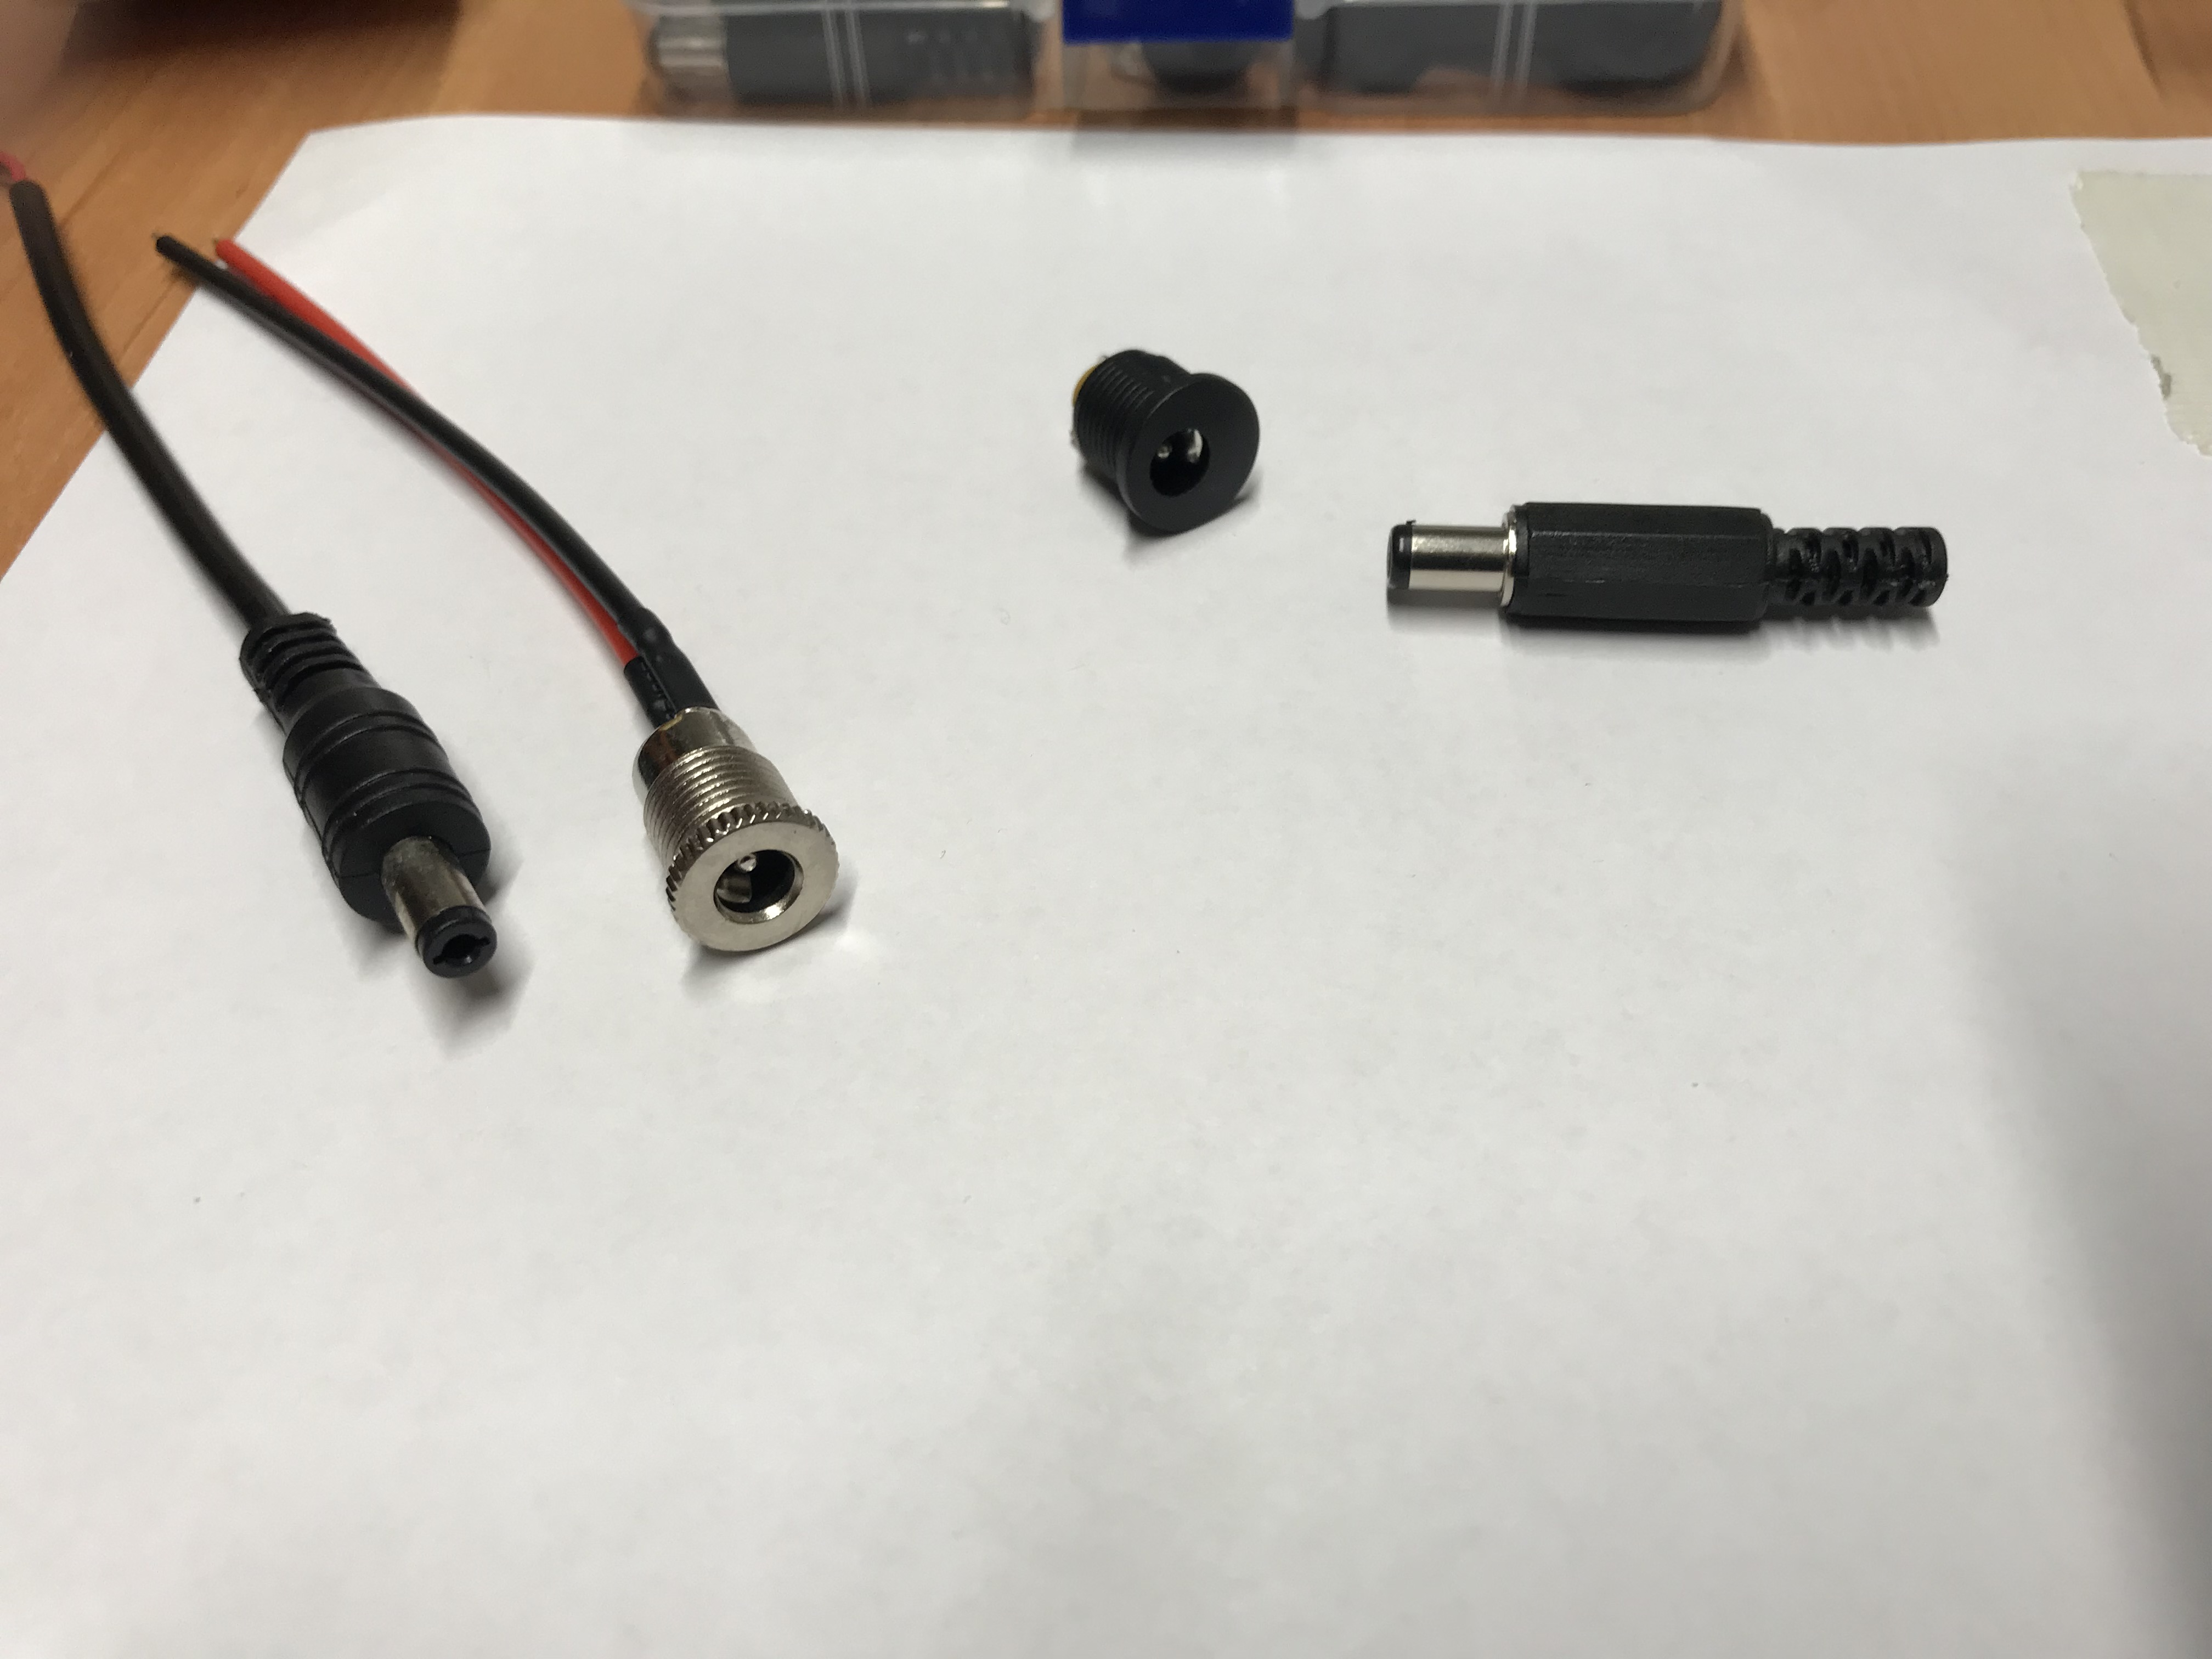
\includegraphics[scale=.07]{pictures/dcJack.jpg}};
            \end{scope}
        }{
            \draw (0,0) rectangle (3,1.5) ;
        }{Amazon}{Sin Id} {24V} {3.5A}
        \cline{1 - 2}
        \multicolumn{5}{|l|}{\makecell[l]{
            \tabitem Incluye tuerca para sujetar a panel \\
            \tabitem Incluye protector de goma
        }} \\
        \hline
    \end{tabular}
    \caption{Jack 2mm Amazon}
    \label{tab:DcJack1}
\end{table}

%DC jack Metal Amazon
\begin{table}[H]
    \centering
    \renewcommand\theadfont{\bfseries}
    \setlength{\tabcolsep}{10pt}
    \renewcommand{\arraystretch}{1.5}

    \begin{tabular}{|c|c|c|c|c|}
        \beginConnectorTable{DC Jack 2mm}
        \multirow{3}{*}{\makecell{Macho \\ Plug}}
    
        \connectordata{
            \begin{scope}
                \clip (-1,-0.65) rectangle  +(2,1.3);
                \node[inner sep=0pt, rotate=60] at (1.3,2)
                    {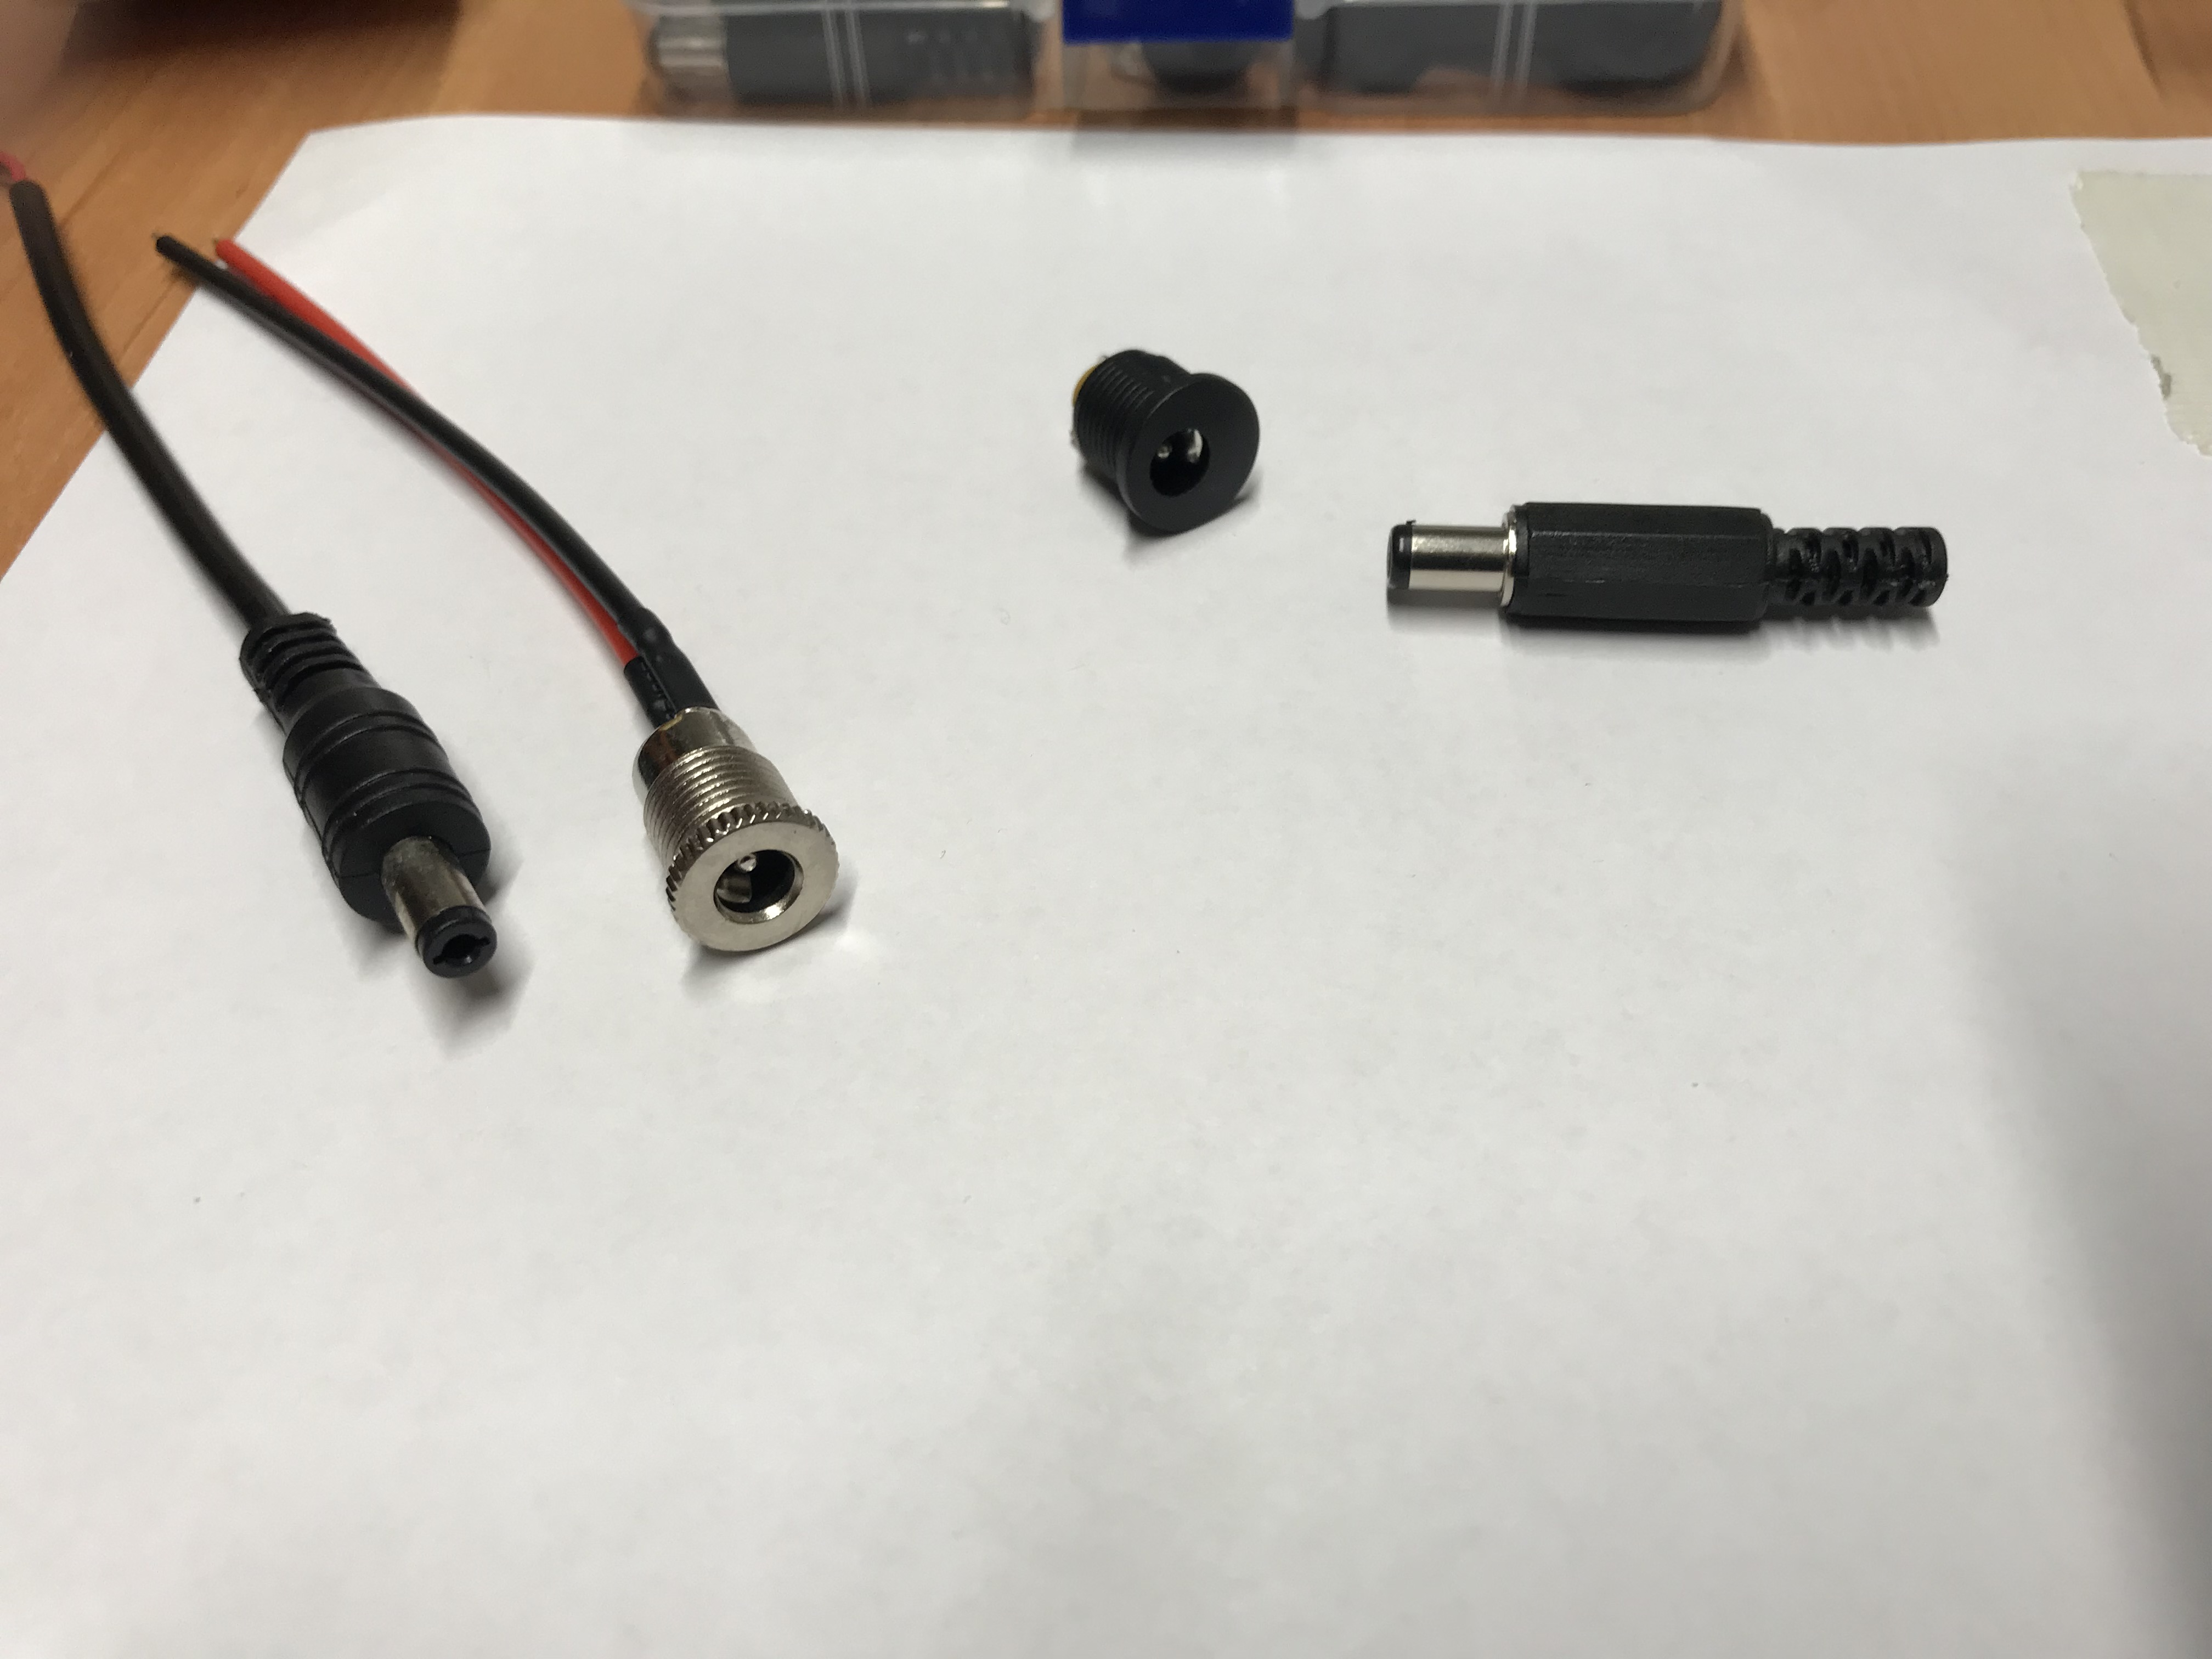
\includegraphics[scale=.05]{pictures/dcJack.jpg}};
            \end{scope}
           
        }{
            \draw (0,0) rectangle (3,1.5) ;
        }{Amazon}{Sin Id} {24V} {3A}
        \cline{1 - 2}
        \multirow{3}{*}{\makecell{Hembra \\ Socket}}
        \connectordata{
            \begin{scope}
                \clip (-1,-0.65) rectangle  +(2,1.3);
                \node[inner sep=0pt, rotate=60] at (0.9,1)
                    {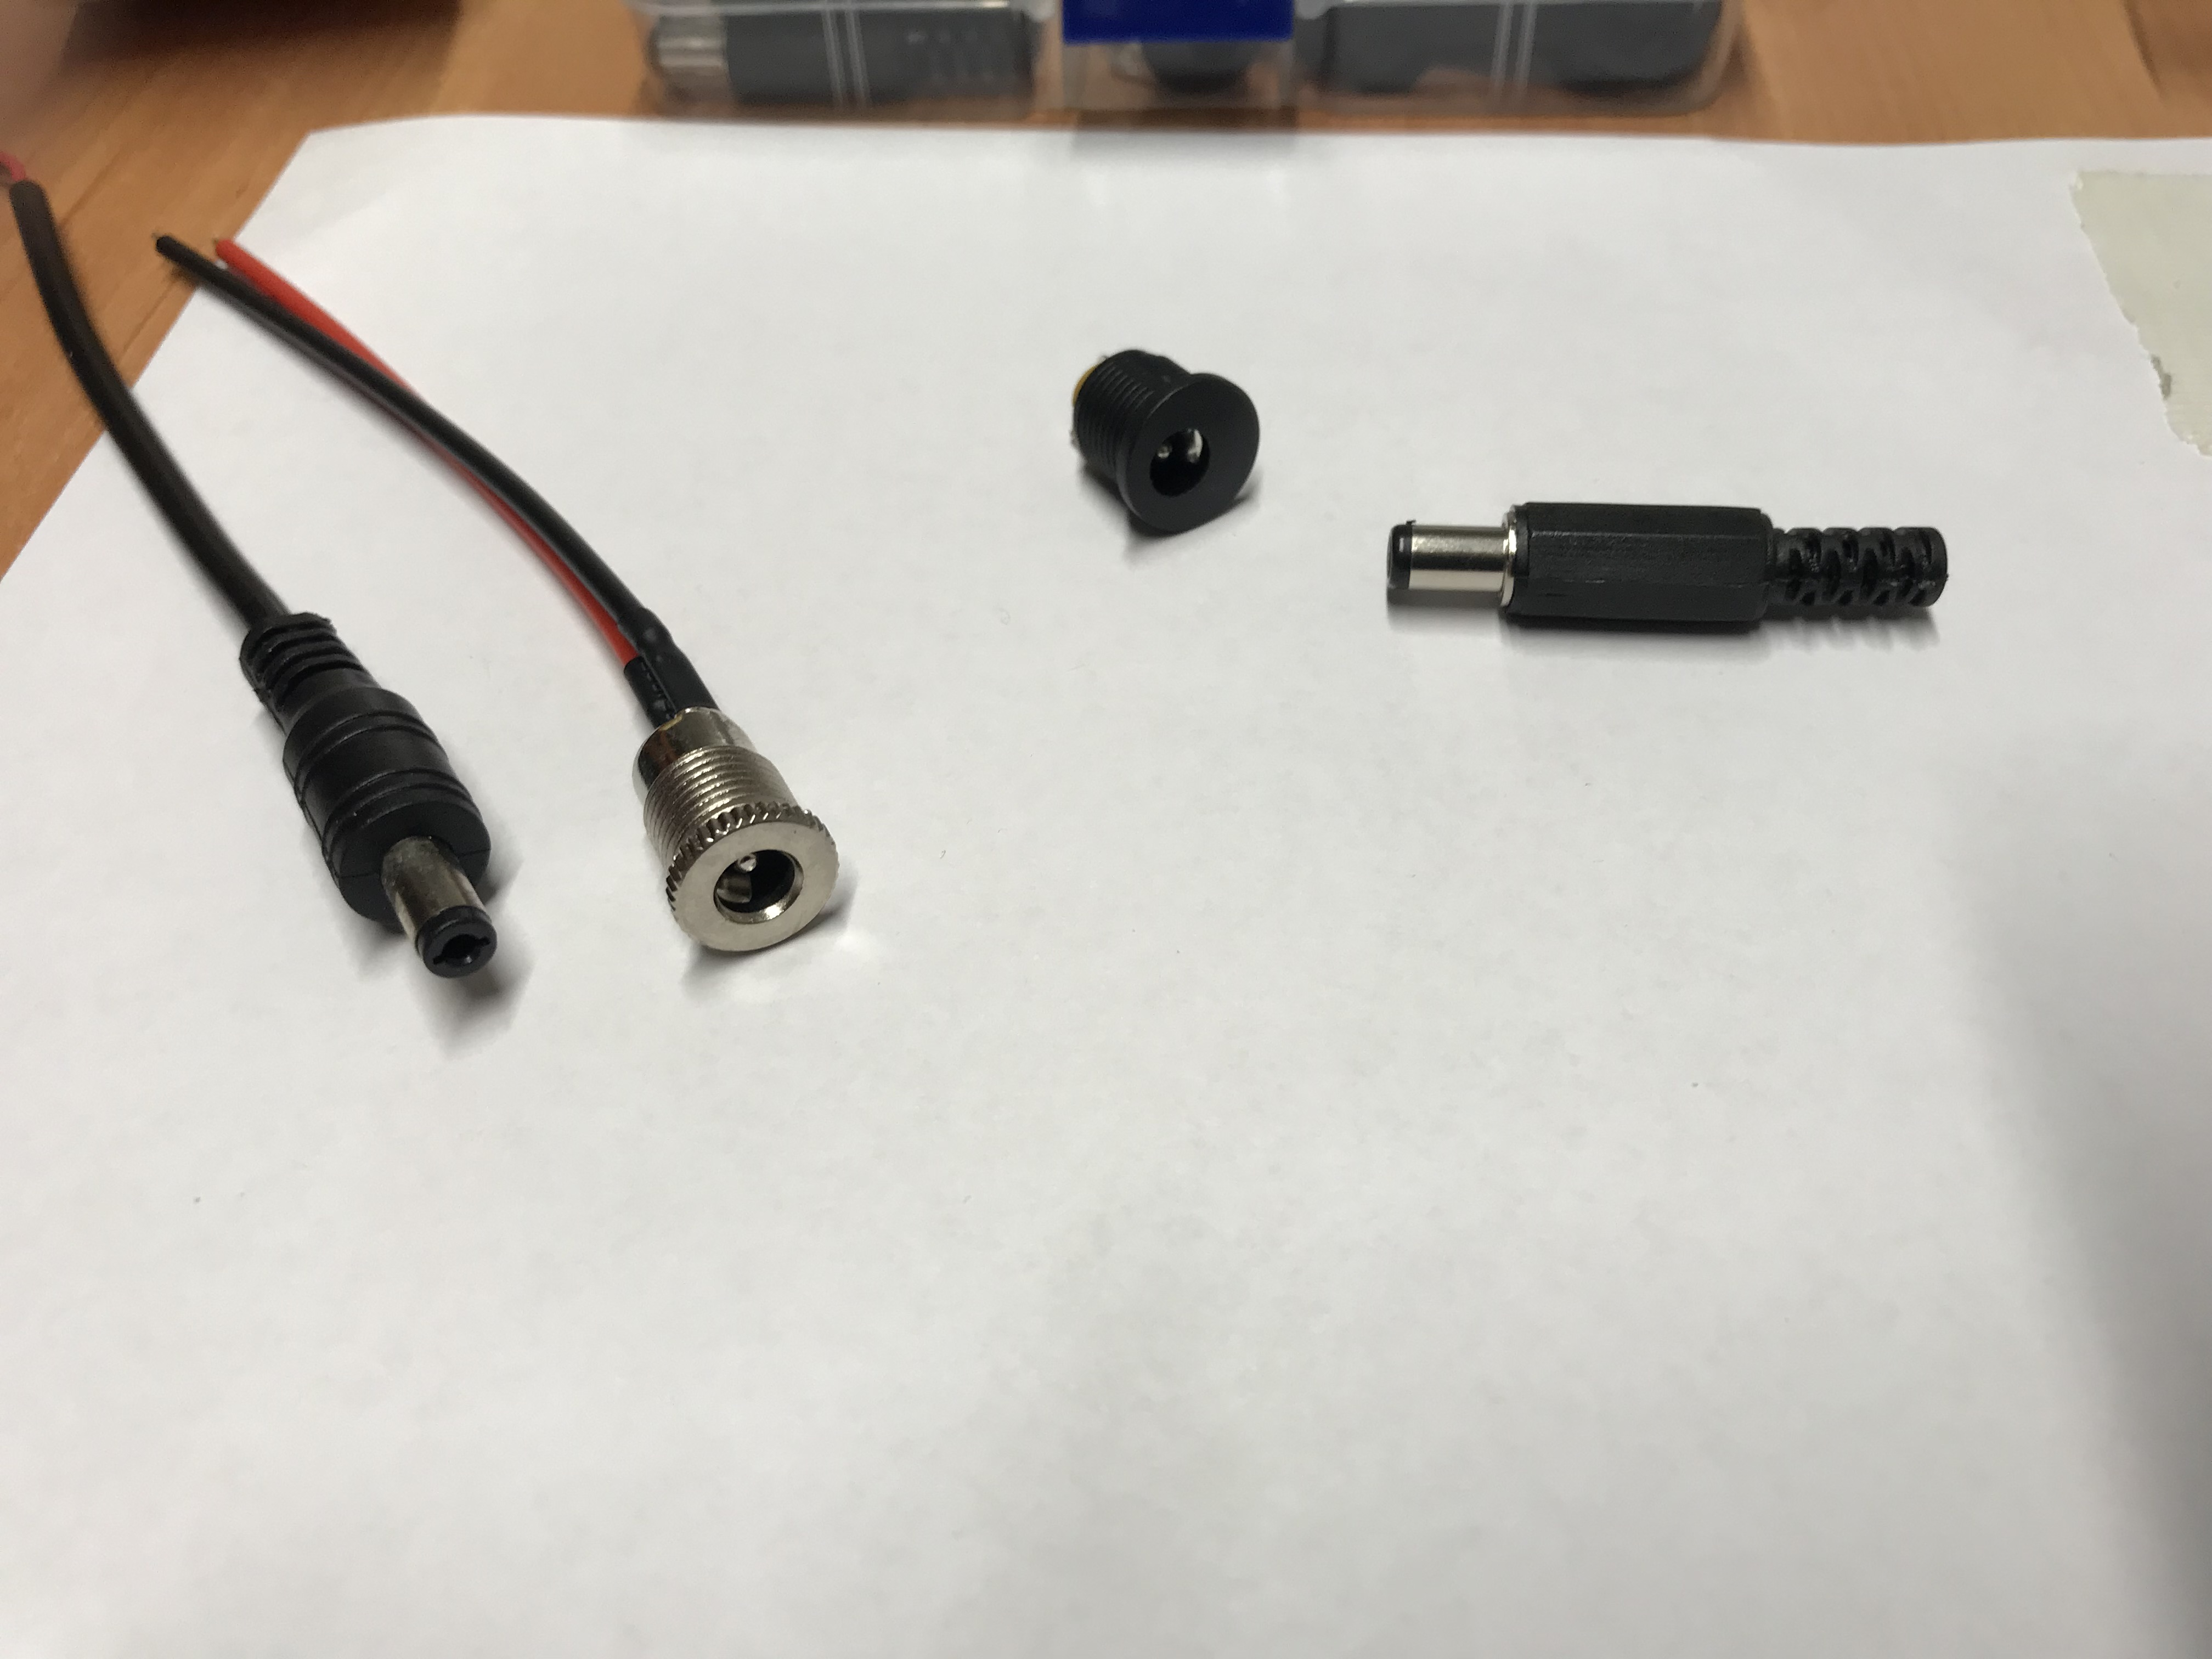
\includegraphics[scale=.05]{pictures/dcJack.jpg}};
            \end{scope}
        }{
            \draw (0,0) rectangle (3,1.5) ;
        }{Amazon}{Sin Id} {24V} {3A}
        \cline{1 - 2}
        \multicolumn{5}{|l|}{\makecell[l]{
            \tabitem Incluye tuerca para sujetar a panel \\
            \tabitem Es de metal conectado a (-) \\
            \tabitem Cables pre-soldados
        }} \\
        \hline
    \end{tabular}
    \caption{Jack 2mm Amazon}
    \label{tab:DcJack2}
\end{table}

%KLDX-0202-A PCB
\begin{table}[H]
    \centering
    \renewcommand\theadfont{\bfseries}
    \setlength{\tabcolsep}{10pt}
    \renewcommand{\arraystretch}{1.5}

    \begin{tabular}{|c|c|c|c|c|}
        \beginConnectorTable{KLDX-0202-A Jack Para PCB}
        \multirow{3}{*}{\makecell{Hembra \\ Socket}}
        \connectordata{
            \begin{scope}
                \clip (-1,-0.75) rectangle  +(2,1.5);
                \node[inner sep=0pt] at (0,0)
                    {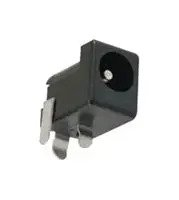
\includegraphics[scale=.35]{pictures/connectors/KLDX-0202-A.jpg}};
            \end{scope}
        }{
            \draw (0,0) rectangle (3,1.5) ;
        }{Mouser}{KLDX-0202-A} {24V} {3A}
        \cline{1 - 2}
        \multicolumn{5}{|l|}{\makecell[l]{
            \tabitem Para PCB
        }} \\
        \hline
    \end{tabular}
    \caption{Jack 2mm PCB}
    \label{tab:DcJackPcb}
\end{table}
